% ..............................................................................
% Demo of the fau-beamer template.
%
% Copyright 2022 by Tim Roith <tim.roith@fau.de>
%
% This program can be redistributed and/or modified under the terms
% of the GNU Public License, version 2.
%
% ------------------------------------------------------------------------------
\documentclass[final]{beamer}

% ========================================================================================
% Theme: inner, outer, font and colors
% ----------------------------------------------------------------------------------------
\usepackage[institute=FAU,
			%SecondLogo = template-art/FAUWortmarkeBlau.pdf,
			%ThirdLogo = template-art/FAUWortmarkeBlau.pdf,
			%WordMark=None,
			aspectratio=169,
			fontsize=11,
			fontbaselineskip=13,
			scale=1.,
			InsertTotalFoot
		   ]{styles/beamerthemefau}
% ----------------------------------------------------------------------------------------
% Input and output encoding
\usepackage[T1]{fontenc}
\usepackage[utf8]{inputenc}
% \usepackage{fontspec}
% ----------------------------------------------------------------------------------------
% Language settings
\usepackage[english]{babel}

% ========================================================================================
% Fonts
% - Helvet is loaded by styles/beamerfonts
% - We use serif for math environements
% - isomath is used for upGreek letters
% ----------------------------------------------------------------------------------------
% \usepackage{isomath}
% \usefonttheme[onlymath]{serif}
% \usepackage{exscale}
% \usepackage{anyfontsize}
\setbeamercolor{alerted text}{fg=BaseColor}
% ----------------------------------------------------------------------------------------
% custom commands for symbols
\usepackage{styles/symbols}


% ========================================================================================
% Setup for Titlepage
% ----------------------------------------------------------------------------------------
\title[Optimizing internal memory representation in Jayvee]{Optimizing internal memory representation in Jayvee}
\subtitle{Bachelor thesis}
\author[J. Zeltner]{
Jonas Zeltner\inst{1}\and%
\inst{2}\and%
\inst{3}%
}
%
\institute[FAU]{%
\inst{1} Friedrich-Alexander-Universität Erlangen-Nürnberg \and%
\inst{2} Faculty of Engineering, Department Computer Science \and%
\inst{3} Professorship for Open Source Software
}

% Instead of \institute you can also use the \thanks command
% ------------------------------------------------
% \author[J. Zeltner]{
% Jonas Zeltner\thanks{Friedrich-Alexander Universität Erlangen-Nürnberg}\and%
% \thanks{Faculty of Engineering, Department Computer Science}\and%
% \thanks{Professorship for Open Source Software}%
% }

\date{24. September 2024}


% ================================================
% Bibliography
% ------------------------------------------------
\usepackage[outputdir=aux]{minted}
% \usemintedstyle{bw}
\usepackage{csquotes}
\usepackage{perpage}
\MakePerPage{footnote}
\usepackage[style=apa,backend=biber]{biblatex}
\addbibresource{bibliography.bib}
\setbeamertemplate{bibliography item}[text]


% ================================================
% Hyperref and setup
% ------------------------------------------------
\usepackage{hyperref}
\hypersetup{
	colorlinks = true,
	final=true,
	plainpages=false,
	pdfstartview=FitV,
	pdftoolbar=true,
	pdfmenubar=true,
	pdfencoding=auto,
	psdextra,
	bookmarksopen=true,
	bookmarksnumbered=true,
	breaklinks=true,
	linktocpage=true,
	urlcolor=BaseColor,
	citecolor=BaseColor,
	linkcolor=BaseColor
}


% ================================================
% Additional packages
% ------------------------------------------------
\usepackage{subcaption}
\usepackage[inkscapelatex=false]{svg}
\usepackage{tikz}
\usepackage{pgfplots}
\pgfplotsset{compat=newest}
\usepackage{listings}
\usepackage{siunitx}

\usepackage{pifont}
\newcommand{\xmark}{\ding{55}}



% ================================================
% Various custom commands
% ------------------------------------------------
%\setbeameroption{show notes on second screen}
\begingroup\expandafter\expandafter\expandafter\endgroup
\expandafter\ifx\csname pdfsuppresswarningpagegroup\endcsname\relax
\else
  \pdfsuppresswarningpagegroup=1\relax
\fi
% Change color for cite locally
\newcommand{\colorcite}[3]{{\hypersetup{citecolor=#1}{\cite[#2]{#3}}}}
% ------------------------------------------------




% ================================================
% The main document
% ------------------------------------------------
\begin{document}
% Title page
\begin{frame}[t,titleimage]{-}
	\titlepage
\end{frame}

\begin{frame}[t]{Introduction}{What is this?}
	This file demonstrates the fau-beamer style, which is a style for the \LaTeX{} \texttt{beamer} class, which allows to create presentation slides in \LaTeX. The design is based on the FAU corporate \href{https://www.intern.fau.de/kommunikation-marketing-und-corporate-identity/corporate-identity/}{ style guide 2021}.

	This code for this template was written by \href{https://timroith.github.io/}{Tim Roith}. If you have questions about the template or found a mistake you can send an email to tim\{dot\}roith\{at\}fau\{dot\}de or open a issue at the \href{https://github.com/FAU-AMMN/fau-beamer}{GitHub repository}.
\end{frame}


\begin{frame}[title]{-}
	\tableofcontents
\end{frame}

\section{Background information} % FIXME: improve name
\begin{frame}[t]{Explanations}{Jayvee}
	\begin{itemize}
		\item \emph{Jayvee}: Language aiming to allow everyone to describe data pipelines \footcite{jvalue:jayvee}.
		      \begin{figure}[h]
			      \begin{center}
				      \includesvg[width=0.5\linewidth]{assets/etl.svg}
			      \end{center}
			      \caption{The basic structure of a pipeline \footcite{jvalue:jayvee:docs:core_concepts}}
		      \end{figure}
		\item<2-> Examples:
		      \begin{description}
			      \item[Extractor] \Verb|HttpExtractor|, \Verb|LocalFileExtractor|
			      \item[Transformer] \Verb|CSVInterpreter|, \Verb|TableTransformer|
			      \item[Loader] \Verb|CSVFileLoader|, \Verb|SQLiteLoader|
		      \end{description}
		\item<3-> \emph{Jayvee} interpreter: Program that can parse \emph{Jayvee} source files and execute the defined pipelines
	\end{itemize}
\end{frame}


\begin{frame}[t]{Explanations}{Columnar storage}
	\begin{columns}[t]
		\begin{column}[t]{0.4\linewidth}
			\begin{itemize}
				\item Approach to represent tables in linear memory
				\item Values are saved column after column\footnotemark
				\item<2-> Advantages over row-oriented storage:
				      \begin{itemize}
					      \item Column specific compression\footnotemark
					      \item Less memory usage\footnotemark[2]
					      \item Faster read times\footnotemark[1]
				      \end{itemize}

			\end{itemize}
		\end{column}
		\hfill
		\begin{column}{0.6\linewidth}
			\begin{figure}
				\centering
				\begin{subfigure}{0.8\linewidth}
					\centering
					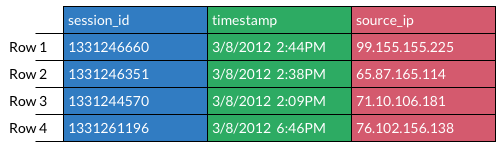
\includegraphics[height=0.2\FrameHeight]{assets/table-example}
					\caption{An example table in \dots}
				\end{subfigure}
				\\
				\begin{subfigure}{0.4\linewidth}
					\centering
					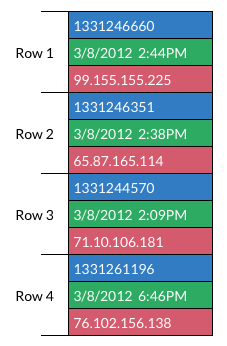
\includegraphics[height=0.3\FrameHeight]{assets/table-row}
					\caption{\dots row-oriented memory.}
				\end{subfigure}
				\begin{subfigure}{0.4\linewidth}
					\centering
					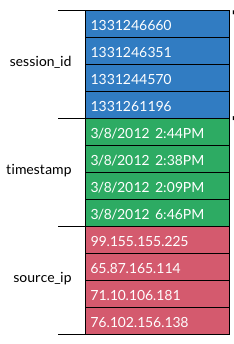
\includegraphics[height=0.3\FrameHeight]{assets/table-columnar}
					\caption{\dots columnar memory.}
				\end{subfigure}
				\caption{A table's is representation in row-oriented and columnar memory\footnotemark[3].}
			\end{figure}
		\end{column}
	\end{columns}
	\footnotetext[1]{\textcite{Floratou2019}}
	\footnotetext[2]{\textcite{Abadi2013}}
	\footnotetext[3]{\textcite{arrow:overview}}
\end{frame}

\begin{frame}[t]{Explanations}{Apache Arrow}
	\begin{columns}[t]
		\begin{column}{0.4\linewidth}
			Apache Arrow specifies:
			\begin{itemize}
				\item A format\footnotemark \text{ }that is:
				      \begin{itemize}
					      \item Columnar
					      \item In-memory
					      \item Language agnostic
				      \end{itemize}
				\item<3-> An IPC file format\footnotemark
			\end{itemize}
		\end{column}
		\hfill
		\begin{column}{0.6\linewidth}
			\centering
			\only<2> {
				\begin{figure}
					\begin{tikzpicture}
						\draw (0,0) -- (12,0)
						(0,1) -- (12,1)
						(0,2) -- (12,2)
						(0,3) -- (12,3)
						(0,4) -- (12,4)
						(0,5) -- (12,5)
						(0,6) -- (12,6)
						(0,7) -- (12,7)
						(0,8) -- (12,8)
						(0,9) -- (12,9)
						(0,0) -- (0,3) (0,4) -- (0,7) (0,8) -- (0,9)
						(3,0) -- (3,3) (3,4) -- (3,7) (3,8) -- (3,9)
						(6,0) -- (6,3) (6,4) -- (6,7) (6,8) -- (6,9)
						(9,0) -- (9,3) (9,4) -- (9,7) (9,8) -- (9,9)
						(12,0) -- (12,3) (12,4) -- (12,7) (12,8) -- (12,9);
						\node[] at (1.5,8.5) {\tiny \textbf{name}: Utf8};
						\node[] at (4.5,8.5) {\tiny \textbf{age}: Int};
						\node[] at (7.5,8.5) {\tiny \textbf{height}: Decimal};
						\node[] at (10.5,8.5) {\tiny \textbf{birth}: Timestamp};
						\draw[orange,thick] (-0.1,7.9) rectangle (12.1,9.1) node[anchor=south east]{\footnotesize schema};
						\draw[blue,thick] (3.2,8.2) -- (5.8,8.2) -- (5.8,8.8) -- (3.2,8.8) -- (3.2,8.2) node[anchor=north west] {\footnotesize field};
						\draw[red,thick] (7.5,8.2) -- (8.8,8.2) -- (8.8,8.8) -- (7.5,8.8) -- (7.5,8.2) node[anchor=north west] {\footnotesize type};
						\draw[teal,thick] (-0.1,3.9) rectangle (3.1,7.1) node[anchor=north west]{\footnotesize array};
						\draw[olive, very thick] (-0.2,3.8) rectangle (12.2,7.2) node[anchor=north east]{\footnotesize record batch};

					\end{tikzpicture}
					\caption{Key concepts of an Arrow table\footnotemark}
				\end{figure}
			}
			\only<3>{
				\begin{figure}
					\centering
					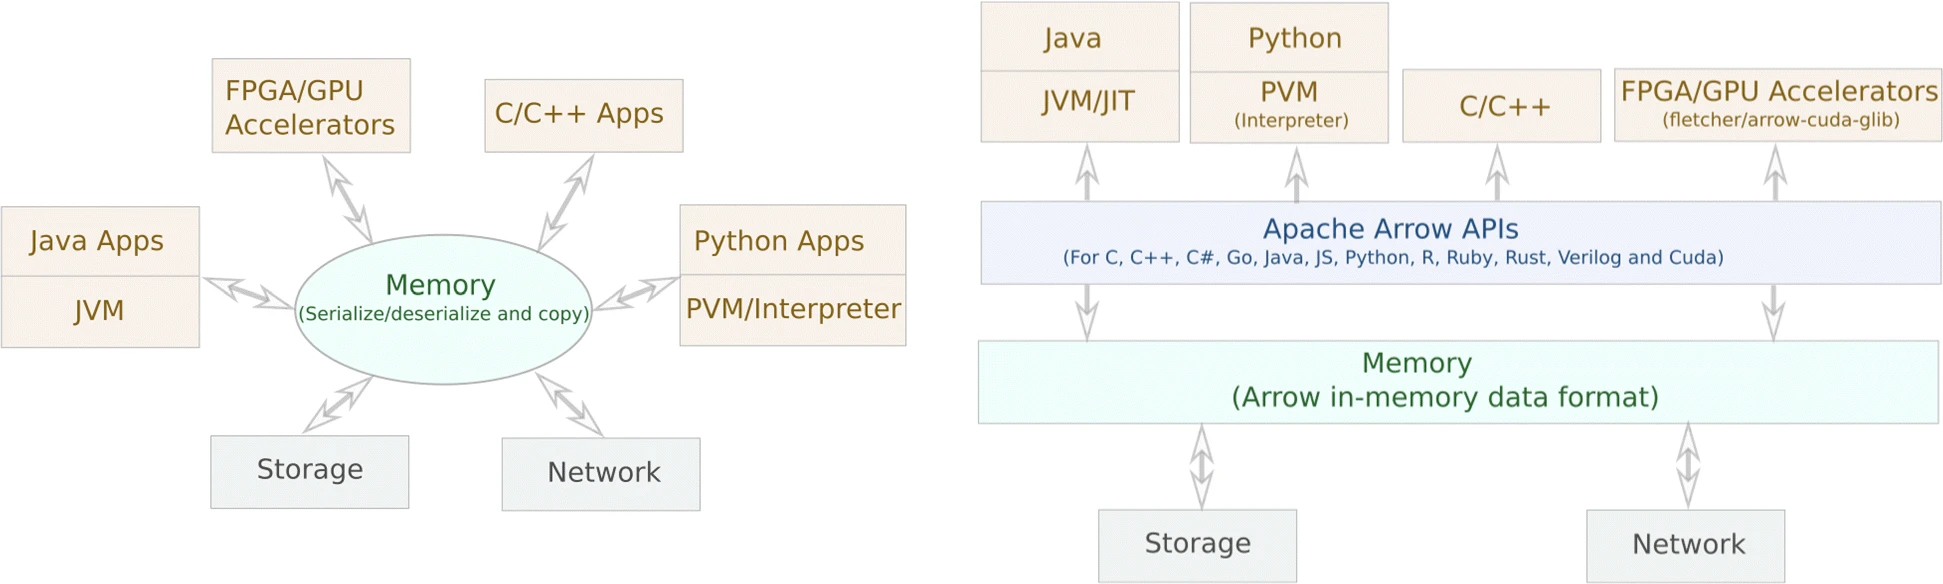
\includegraphics[width=0.9\linewidth]{assets/arrow_interop.png}
					\caption{How \emph {Arrow} enhances interoperability between modules}
				\end{figure}
			}
		\end{column}
		\hfill
	\end{columns}
	\footnotetext[1]{\textcite{arrow:spec}}
	\footnotetext[2]{\textcite{arrow:spec:ipc}}
	\footnotetext[3]{\textcite{Dremio}}
\end{frame}





\begin{frame}[allowframebreaks]{References}
	% \begin{block}{References}
	\printbibliography[heading=none]
	% \end{block}
\end{frame}

\end{document}
